%\makeatletter\let\ifGm@compatii\relax\makeatother
\documentclass[pdftex,12pt,xcolor=pdftex,table]{beamer}
%\documentclass[handout,12pt,xcolor=pdftex,table]{beamer}
\synctex=1
\usepackage{comment}
\usepackage{etex}
\usepackage{amsmath}
\usepackage{amsthm}
\usepackage{amsfonts}
\usepackage{amssymb}
\usepackage{latexsym}
\usepackage{mathtools}
\usepackage[utf8]{inputenc}
\usepackage{tikz}
\usetikzlibrary{calc,matrix,shapes,arrows}
\usepgflibrary{shapes.arrows}
\usepackage[nomessages]{fp}% http://ctan.org/pkg/fp
\newcounter{mycols}
\usepackage[]{graphicx}
\usepackage[sort]{natbib}
\usepackage{bibentry}
\usepackage{booktabs}
%\usepackage{omer}
\usepackage{layout}
\usepackage[justification=centering,figureposition=bottom]{caption}
\usepackage{longtable}
\usepackage{lscape}
\usepackage{rotating}
\usepackage[figtopcap,center,scriptsize]{subfigure}%[figtopcap]
\usepackage{appendix}
\usepackage{setspace}
\usepackage[multiple,stable]{footmisc}
\captionsetup[longtable]{width=.75\textwidth}

\DeclareGraphicsExtensions{.png,.pdf}
\DeclareTextFontCommand{\emph}{\bfseries}
%% THEOREMS -------------------------------------------------------
\newtheorem{thm}{Theorem}[section]
\newtheorem{cor}[thm]{Corollary}
\newtheorem{lem}[thm]{Lemma}
\newtheorem{prop}[thm]{Proposition}
\theoremstyle{definition}
\newtheorem{defn}[thm]{Definition}
\theoremstyle{remark}
\newtheorem{rem}[thm]{Remark}
\numberwithin{equation}{section}
%
%% MATH -----------------------------------------------------------
\newcommand{\set}[1]{\left\{#1\right\}}
\newcommand{\eps}{\varepsilon}
\newcommand{\To}{\longrightarrow}

\newcounter{panel}[table]
\renewcommand{\thepanel}{\Alph{panel}}
\newcommand{\mypanel}[1][]{\refstepcounter{panel}Panel \thepanel: \ #1}

\newenvironment{stepenumerate}{\begin{enumerate}[<+->]}{\end{enumerate}}
\newenvironment{stepitemize}{\begin{itemize}[<+->]}{\end{itemize} }
%\newenvironment{stepitemize}{\begin{itemize}}{\end{itemize} }
\newenvironment{stepenumeratewithalert}{\begin{enumerate}[<+-| alert@+>]}{\end{enumerate}}
\newenvironment{stepitemizewithalert}{\begin{itemize}[<+-| alert@+>]}{\end{itemize} }
\newtheorem{assumption}{Assumption}
\newtheorem{proposition}{Proposition}
\usetheme{CambridgeUS}
\setbeamertemplate{navigation symbols}{}
\numberwithin{figure}{section}

\makeatletter
\let\@@magyar@captionfix\relax
\makeatother

\usepackage{multicol}


\tikzset{arrowcases/.style={matrix anchor=west,%
  nodes={anchor=base west,%
         name=arrc-\the\pgfmatrixcurrentrow-\the\pgfmatrixcurrentcolumn},%
  execute at begin cell=\node\bgroup\math\displaystyle,%
  execute at end cell=\endmath\egroup;,%
  ampersand replacement=\&}}

\def\beginarrowcases#1\endarrowcases{
\begin{tikzpicture}[baseline=(O)]
  \matrix [arrowcases] {
  #1
  };
  \coordinate (A) at (arrc-1-1.west);
  \coordinate (B) at (arrc-\the\pgfmatrixcurrentrow-1.west);
  \coordinate (start) at ($(A)!0.5!(B) - (5em,0)$);
  \foreach \nn in {1,...,\pgfmatrixcurrentrow} {
    \draw[double, -triangle 45,<->] ($(start)+(0,1.5em - \nn em)$) -- (arrc-\nn-1.west);
  };
  \coordinate (O) at ($(start)-(0,0.5ex)$);
  \node at (-1em,0) {};
\end{tikzpicture}}



\documentclass[11pt]{beamer}
\usepackage[utf8]{inputenc}
\usepackage[spanish]{babel}
\usepackage{amsmath}
\usepackage{amsfonts}
\usepackage{amssymb}
\usepackage{graphicx}
\usepackage{lipsum}
\usepackage{ragged2e}
\usepackage{hyperref}
\usepackage{float}
\usepackage{url}
\usetheme{CambridgeUS}
\newcommand{\celda}[1]{
	\begin{minipage}{2.5cm}
		\vspace{5mm}
		#1
		\vspace{5mm}
	\end{minipage}
}

\author[Ana Maestre & Daniela Sayago]{Ana Paulina Maestre \inst &\&  Daniela Sayago}
\title[This mine is mine!]{This mine is mine!}
\date{June 2020} 
\subtitle{ how minerals fuel conflicts in africal}
\institute[PUJ]{
	\inst{}
		Pontifical Javeriana University. Faculty of Economic and Administrative Sciences. \\Economic Growth and Comparative Development \\
		\vspace{2mm}

}

\AtBeginSection[]
{
	\begin{frame}<beamer>{Content}
		\tableofcontents[currentsection,currentsubsection]
	\end{frame}
}


\begin{document}
	
	\begin{frame}
		\maketitle
	\end{frame}

	\begin{frame}{content}
		\tableofcontents
	\end{frame}

	\section{Conceptual Framework}
		\begin{frame}{Existing Evidence and Conceptual Framework}
			\justifying
\item - Civil wars have positive correlation with natural resources
\item - Resources increase feasibility
\item - Weak state capacity 
\item - Impact of higher local income
\item - Role of foreign companies
		\end{frame}
		
	
	\section{Data}
		\begin{frame}{Data}
			\justifying
\item 1. Data			
\item 1.1 Conflict data
\item 1.2 Mines data
\item 1.3 Other data
\item 2. Descriptive statistics
		\end{frame}
		
		\begin{frame}{Conflict Data}
			\justifying
\item - Armed Conflict Location Events Data
\item - Dummy variable= 1 when at least one event of conflict has occurred inside the given cell
\item - Bias due to coverage of conflict
		\end{frame}
	
	\begin{frame}{Mines Data}
			\justifying
\item - Raw Material Data
\item - Mkt= 1 when at least one mine is active inside the given cell during a given year
\item - Mkt: proxy to extraction area of a certain mineral
\item - Bias due to lack of data on small mines
		\end{frame}
		
			\begin{frame}{Other Data}
			\justifying
\item - World Bank Commodities
\item - Excluding diamonds
\item - Include:
    \item cell-specific variables 
    \item country-specific variables
    \item mineral-specific variables
		\end{frame}
		
		 \begin{frame}{Descriptive Statistics}
        \justifying
        \begin{figure}[H]
				\centering
				\includegraphics[scale=0.45]{Tabe 1.png}
			\end{figure}
			\end{frame}
		
		\begin{frame}{Descriptive Statistics}
			\justifying
\item - 52 countries, 14 minerals
\item - Main minerals
\item - The conflict probability is much higher in cells with active mines, around 14 percent
\item - The presence of active mines is positively correlated with conflict incidence, both across and within cells
		\end{frame}
	
	\section{Empirical Analysis}
		\begin{frame}{Empirical Analysis}
			\justifying

\item 1. Methodological Issues
\item 2. Baseline Results
\item 3. Sensitivity Analysis 
\item 4. Country Characteristics and Mining-Induced Violence 
\item 5. Mineral Characteristics
\item 6. The Nature of Mining-Induced Violence
\item 7. Quantification

    
		\end{frame}
		
		\begin{frame}{Methodological Issues}
			\justifying
 	         More valuable mines increase the search for local rents, leading to a higher probability of violence.
  \[CONFLICT_{kt}= \alpha_{1} M_{kt}+ \alpha_{2}ln P^w_{kt}+ \alpha_{3}(M_{kt}xln P^w_{kt})+ FE_{k}+FE_{it}+\epsilon_{kt}\]  
  
	\begin{itemize}
\item \alert{FEkt}  are cell fixed effects
\item \alert{FEit} is an additional battery of fixed effects 
\item \alert{Conflictkt}   is the dependent variable
\item \alert{Mkt}  is the main explanatory variable
\item \alert{pkt} w is the variable corresponds to the world price in year t 

    \end{itemize}	         

        \end{frame}

	    \begin{frame}{Methodological Issues: Significant Factors}
			\justifying
 	        \textbf {1. Exogeneity of Prices:}
            \begin{itemize}
            \item Some mines may be large enough to affect world prices; if a conflict were to occur in mining areas, prices could be affected.
            \item Omitted variables that vary over time could determine world prices and local violence in mining areas.
    \end{itemize}
\vfill 

            \textbf {2. Endogenous Mining Activity.}

            \[ CONFLICT_{kt}=  \alpha_{3}(M_{kt}xln P^w_{kt})+ FE_{k}+FE_{it}+\epsilon_{kt}\]  
            
    \end{frame}
 
 
 	    \begin{frame}{Methodological Issues: Significant Factors}
			\justifying
            \textbf {3. Estimation Issues:}
            Equations (1) and (2) were estimated using a Linear Probability Model in the reference specifications.
    \vfill 
            \textbf {4. Spatial Correlation:}
            Given the high spatial resolution of the data, it is important to take spatial correlation into account since both conflict and mines are clustered in space. 
   \end{frame}
   
        \begin{frame}{Baseline Results}
        \justifying
        \begin{figure}[H]
				\centering
				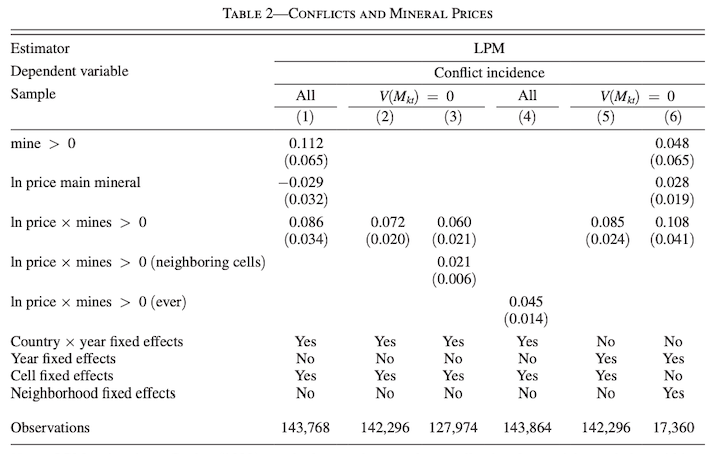
\includegraphics[scale=0.45]{tabla2.png}
				
		\end{figure}
   
 
    \end{frame}
  
        \begin{frame}{Sensitivity Analysis}
        \begin{block}{Sensitivity controls}
             \justifying
        \begin{itemize}
        \item Mining Activity
        \item Main Mineral and Mineral Prices
        \item Alternative Definitions of Violence
        \item Other Robustness Checks

    \end{itemize}
    \end{block}
  
  
    \end{frame}
    
        \begin{frame}{Sensitivity Analysis}
            \justifying
            \begin{itemize}
             \item Mining Activity
         \end{itemize}
         
        \begin{figure}[H]
				\centering
				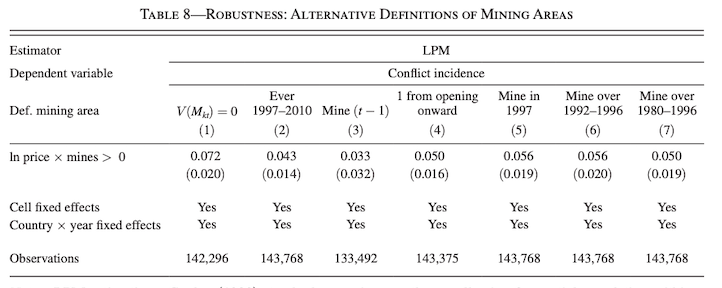
\includegraphics[scale=0.45]{tabla 8.png}
				
			\end{figure}
     \end{frame}
     
         \begin{frame}{Sensitivity Analysis}
            \justifying
         \begin{itemize}
         \item Main Mineral and Mineral Prices
         \vfill 
         \item Other Robustness Checks
         \end{itemize}
         \end{frame}
         
         \begin{frame}{Sensitivity Analysis}
        \begin{itemize}
        \item Alternative Definitions of Violence
        \end{itemize}
         \begin{figure}[H]
				\centering
				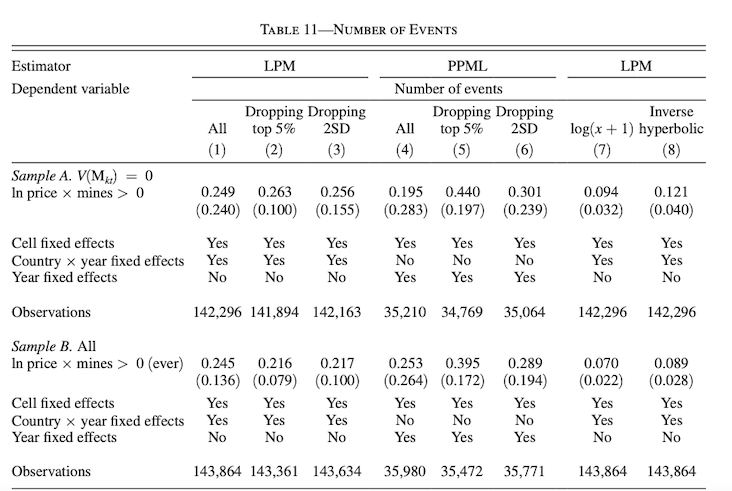
\includegraphics[scale=0.4]{tabla 11.png}
				
			\end{figure}
        
        \end{frame}
         
    \begin{frame}{Country Characteristics and Mining-Induced Violence}
        \justifying
         Is the abundance of valuable mines always a curse for political stability?
        \begin{itemize}
          \item Inequality and Diversity: How Does the Social Fabric Matter
          \end{itemize}
          \vfill 
\item (i) The Gini index of gross income distribution
\item (ii) Ethnic and religious division or polarization
\item (iii) The presence of an indigenous group in the cell
          
    \end{frame}
    
    \begin{frame}{Country Characteristics and Mining-Induced Violence}
    \justifying
    \begin{figure}[H]
				\centering
				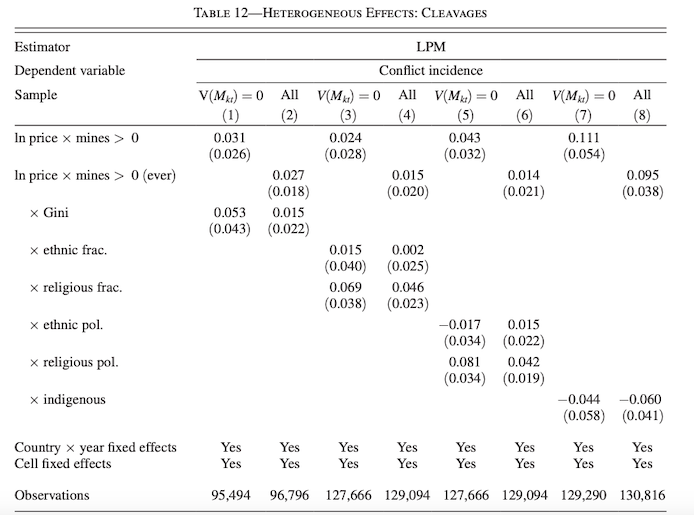
\includegraphics[scale=0.41]{tabla 12.png}
				
			\end{figure}
    
        \end{frame}
    
    \begin{frame}{Country Characteristics and Mining-Induced Violence}
        \justifying
        \begin{itemize}
        \item Domestic Institutions: Can Good Governance Stop the Guns?
        \end{itemize}
        \begin{figure}[H]
				\centering
				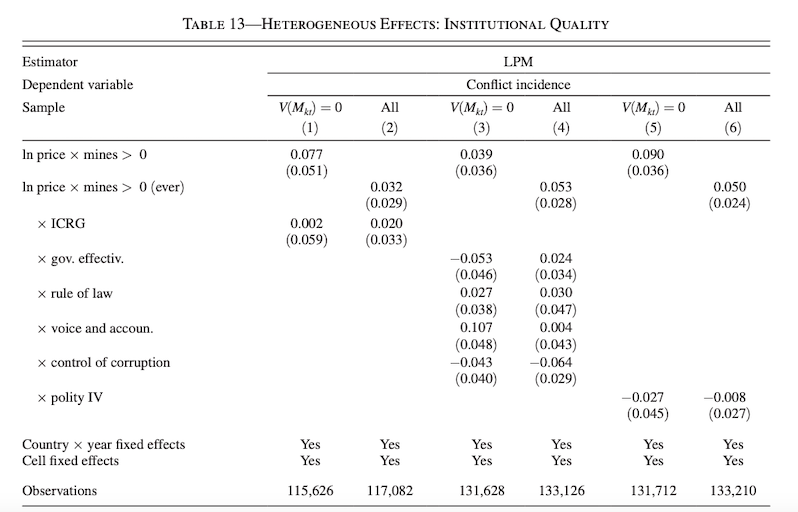
\includegraphics[scale=0.38]{tabla 13.png}
				
			\end{figure}
    
    
        \end{frame}
        
    \begin{frame}{Mineral Characteristics}
        \justifying
        \begin{itemize}
        \item Labor- versus Capital-Intensiveness
        \end{itemize}
        \begin{figure}[H]
				\centering
				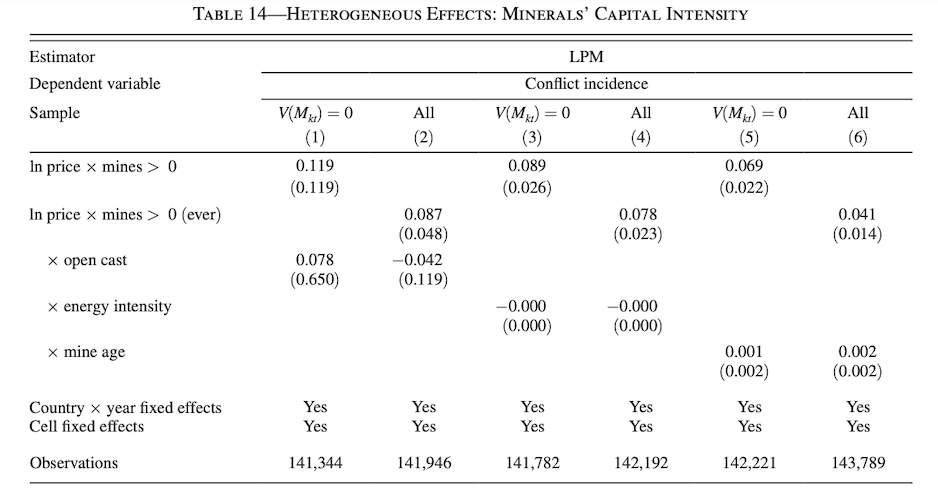
\includegraphics[scale=0.37]{tabla 14.png}
				
			\end{figure}
    
         \end{frame}
         
         \begin{frame}{Mineral Characteristics}
        \justifying
        \begin{itemize}
        \item Rents, Lootability, and Bulkiness
        \end{itemize}
        \begin{figure}[H]
				\centering
				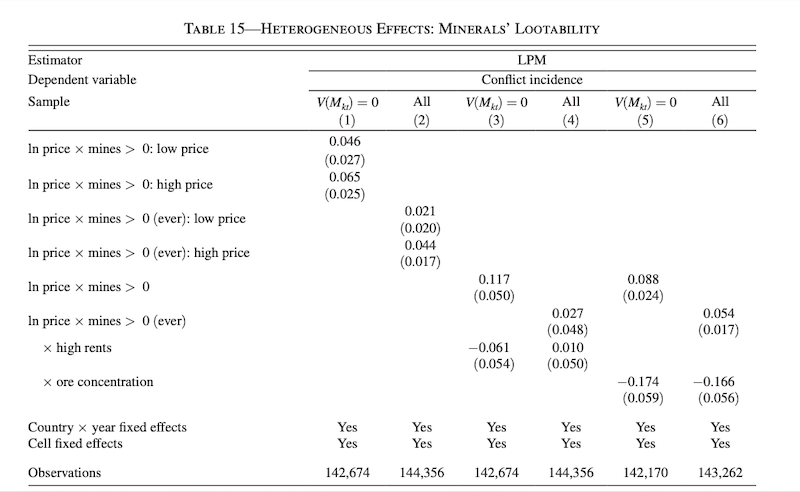
\includegraphics[scale=0.38]{tabla 15.png}
				
			\end{figure}
    
         \end{frame}
         
         \begin{frame}{The Nature of Mining-Induced Violence}
        \justifying
        
        \begin{figure}[H]
				\centering
				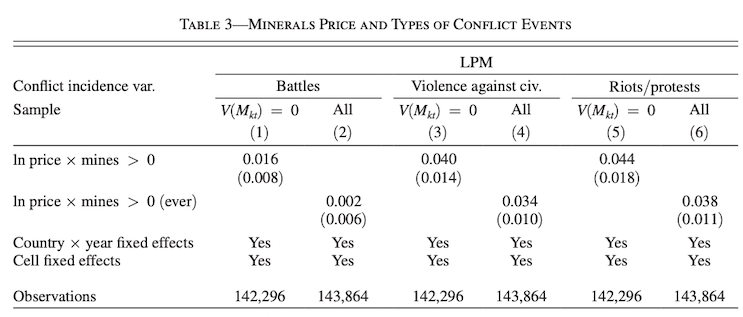
\includegraphics[scale=0.45]{tabla 3.png}
				
			\end{figure}
    
         \end{frame}

    \begin{frame}{Quantification}
        \justifying
        How large is the effect of mineral price variations on the  probability of conflict?  
        \begin{figure}[H]
				\centering
				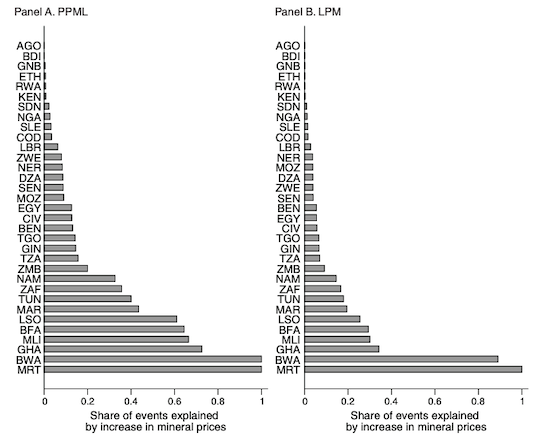
\includegraphics[scale=0.4]{figura1.1.png}
			
				
			\end{figure}
    
         \end{frame}
	
	\section{Feasibility and diffusion of Violence}
		\begin{frame}{Feasibility and the Diffusion of Violence}
			\justifying
\item A) Mines located in ethnic homelands
\item B) Changes in territory
		\end{frame}
		
	
		\begin{frame}{Mines Located in Ethnic Homelands}
			\justifying
\item - How conflict incidence at the rebel group-country level is affected by mineral prices in the ethnic homeland of the group 
\item - Unit of analysis is a rebel group × country of operation × year triplet (g, i, t)
        \end{frame}


\begin{frame}{Mines Located in Ethnic Homelands}
	\begin{figure}[H]
				\centering
				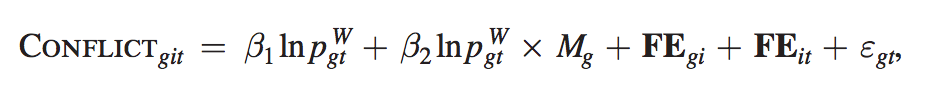
\includegraphics[scale=0.3]{CONFLICT GIT.png}
				\justifying
		\begin{itemize}	
\item \alert{Conflict git} dummy coding for the incidence of a conflict involving group g in country of operation i during year t
\item \alert{ln pw} world price of the main mineral produced by mines located in the homeland of the main ethnicity of rebel group g (the mineral observed in the largest number of cells
\item \alert{Mg} number of mines producing this mineral in the homeland at the beginning of the period
\item \alert{B2} proxy for the mining-related financial capacity of the group 
\end{itemize}
         \end{figure}
    \end{frame}
		
		
		\begin{frame}{Changes in Territory}
			\justifying
\item - The idea is to test whether a change in territory has more effect on future rebel activity elsewhere if the territory is a mining area
			\begin{figure}[H]
				\centering
				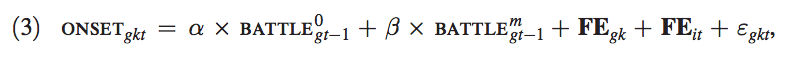
\includegraphics[scale=0.4]{CHANGE.png}
				\justifying
		\begin{itemize}		
\item \alert{ONSETgkt} binary variable equal to 1 if group g is involved in an event in year t in a cell k that was at peace in t − 1; it is 0 if the cell is still in peace in year t
\item \alert{BATTLEm} total number of battles won by group g in t − 1 in mining areas
\item \alert{FEit}country of operation x year xed effects
\item \alert{FEgk} group x cell xed effects
  \end{itemize}
			\end{figure}
		\end{frame}
	
	\section{Breaking the Resource Curse: The Role of Mining Companies}
		\begin{frame}{Breaking the Resource Curse: The Role of Mining Companies}
			\justifying
\item A) Companies' characteristics: Does Mine Ownership Matter?
\item B) Promoting Good Practices: Does Transparency Matter?
	\end{frame}
	

		\begin{frame}{Companies' Characteristics: Does Mine Ownership Matter?}
			\justifying
			\begin{itemize}
            \item Conflict may be escalated by companies propensity to finance
            \item Colonial ties
            \item Firms from the ex-colonizing power continue to benefit from privileged relationships with the new rulers after decolonization
            
            \end{itemize}
            
	        \end{frame}
	        
	        
		\begin{frame}{Promoting Good Practices: Does Transparency Matter?}
			\justifying
			\begin{itemize}
            \item Transparency and traceability
            \item No hard evidence on conflict diminishing
            \item Corporate Social Responsibility
            
            \end{itemize}
            
	        \end{frame}
	   
	
	  \section{Conclusion}
    \begin{frame}{Conclusion}
        \justifying
        \begin{itemize}
        \item Impact of mining activities on the probability of conflict incidence
        \item The sharp increase in mineral prices and the average violence observed in African countries
        \item The results contradict configurations that claim that natural resources can reduce conflict by generating higher local incomes
        \item Mines operated by companies that comply with CSR were found to have less risk of fueling violence
        \item Gaining territorial control of a mining area implications on violencethe diffusion by rebel group
    
        \end{itemize}
        
    
         \end{frame}
         
	

%\appendix
%\subsection<presentation>*{References}

\begin{frame}{References}

\begin{thebibliography}{10}

	
	\bibitem{Author1990}
	 Berman Nicolas, Couttenier Mathieu, Rohner Dominic,
    and Thoenig Mathias.
	\newblock{\em This Mine is Mine! How Minerals Fuel Conflicts in Africa}.
	\newblock{American Economic Review 2017}
	
	

	
	
\end{thebibliography}
\end{frame}
\end{document}

